The term classical computing in this document refers to Von-Neumann serial machines. This approach has brought modern day wonders like personal computers that ease the tasks like writing a novel, calculate incomes and expenses, watch films or talk to relatives living far away. 

As central processing units (CPUs) achieve higher clock frequencies their power consumption increases as well. This is commonly mitigated because newer generations are usually manufactured using smaller transistors, and since they need less power to operate the whole processor consumes less energy. The technology to manufacture such machines is now reaching physical limits and performance is not increasing as expected. One solution to this is to pack multiple processing cores in a single computing unit and run tasks in parallel, which has alleviated the performance hunger for the time being (Figure~\ref{fig:comp:moore}). 

\begin{figure}
  \begin{center}
    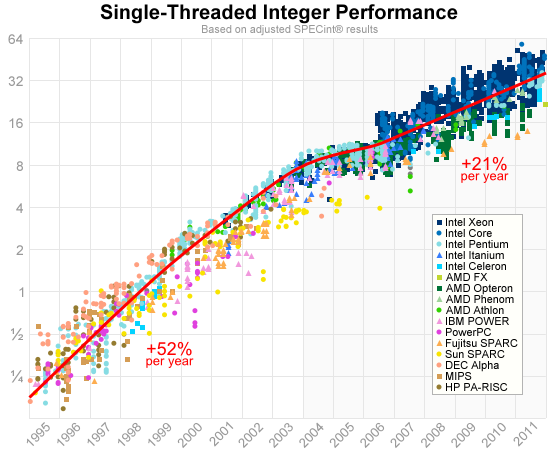
\includegraphics[width=0.6\textwidth]{integer-perf}
    \caption{Performance of CPUs vs release year, a steady increase is observed until about 2004, after that computing platforms where almost forced to use parallel processing~\cite{int-perf-images}. }
    \label{fig:comp:moore}
  \end{center}
\end{figure}